% -*- latex -*-
%%%%%%%%%%%%%%%%%%%%%%%%%%%%%%%%%%%%%%%%%%%%%%%%%%%%%%%%%%%%%%%%
%%%%%%%%%%%%%%%%%%%%%%%%%%%%%%%%%%%%%%%%%%%%%%%%%%%%%%%%%%%%%%%%
%%%%
%%%% This text file is part of the source of 
%%%% `Parallel Programming in MPI and OpenMP'
%%%% by Victor Eijkhout, copyright 2012-2022
%%%%
%%%% debug.tex : tutorial about parallel debugging
%%%%
%%%%%%%%%%%%%%%%%%%%%%%%%%%%%%%%%%%%%%%%%%%%%%%%%%%%%%%%%%%%%%%%
%%%%%%%%%%%%%%%%%%%%%%%%%%%%%%%%%%%%%%%%%%%%%%%%%%%%%%%%%%%%%%%%

\index{debugging|(}

When a program misbehaves, \emph{debugging} is the process of finding
out \emph{why}.
There are various strategies of finding errors in a program.
The crudest one is debugging by print statements. If you have a
notion of where in your code the error arises, you can edit your code
to insert print statements, recompile, rerun, and see if the output
gives you any suggestions. There are several problems with this:
\begin{itemize}
\item The edit/compile/run cycle is time consuming, especially since
\item often the error will be caused by an earlier section of code,
  requiring you to edit, compile, and rerun repeatedly. Furthermore,
\item the amount of data produced by your program can be too large to
  display and inspect effectively, and
\item if your program is parallel, you probably need to print out data
  from all proccessors, making the inspection process very tedious.
\end{itemize}

For these reasons, the best way to debug is by the use of an
interactive \indexterm{debugger}, a program that allows you to monitor
and control the behaviour of a running program. In this section you
will familiarize yourself with
\emph{gdb}\index{GNU!gdb|see{gdb}}, which is the open source
debugger of the \indexterm{GNU} project. Other debuggers are
proprietary, and typically come with a compiler suite. Another
distinction is that gdb is a commandline debugger; there are
graphical debuggers such as \indexterm{ddd} (a~frontend to gdb) or
\indexterm{DDT} and \indexterm{TotalView} (debuggers for parallel
codes). We limit ourselves to gdb, since it incorporates the basic
concepts common to all debuggers.

In this tutorial you will debug a number of simple programs with
gdb and valgrind. The files can be found in the repository
in the directory \n{tutorials/debug_tutorial_files}.
%\n{http://tinyurl.com/ISTC-debug-tutorial}.

\Level 0 {Parallel debugging}

Debugging parallel programs is harder than than sequential
programs, because every sequential bug may show up, plus a number
of new types, caused by the interaction of the various processes.

Here are a few possible parallel bugs:
\begin{itemize}
\item Processes can \indexterm{deadlock} because they are waiting for
  a message that never comes. This typically happens with blocking
  send/receive calls due to an error in program logic.
\item If an incoming message is unexpectedly larger than anticipated,
  a memory error can occur.
\item A collective call will hang if somehow one of the processes does
  not call the routine.
\end{itemize}

There are few low-budget solutions to parallel debugging. The main one
is to create an xterm for each process. We will describe this next.
There are also commercial packages such as \indexterm{DDT} and
\indexterm{TotalView}, that offer a GUI. They are very convenient but
also expensive. The \indexterm{Eclipse} project has a parallel package, 
\indextermbus{Eclipse}{PTP}, that includes a graphic debugger.

\begin{figure}[ht]
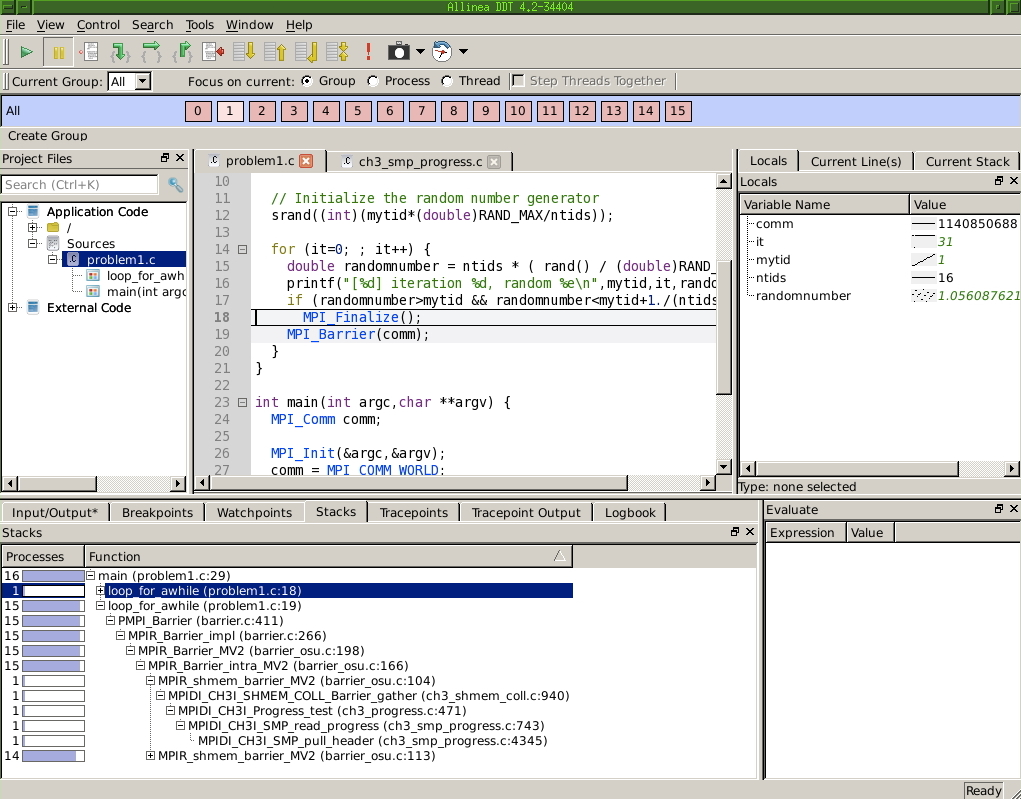
\includegraphics[scale=.4]{ddt2}
\caption{Display of 16 processes in the DDT debugger.}
\label{fig:ddt2}
\end{figure}

Debugging in parallel is harder than sequentially, because you will run
errors that are only due to interaction of processes such as \indexterm{deadlock};
see section~\HPSCref{sec:nonblocking}.

As an example, consider this segment of MPI code:
\begin{verbatim}
MPI_Init(0,0);
// set comm, ntids, mytid
for (int it=0; ; it++) {
  double randomnumber = ntids * ( rand() / (double)RAND_MAX );
  printf("[%d] iteration %d, random %e\n",mytid,it,randomnumber);
  if (randomnumber>mytid && randomnumber<mytid+1./(ntids+1))  
    MPI_Finalize();
}
MPI_Finalize();
\end{verbatim}
Each process computes random numbers until a certain condition is satisfied, then exits.
However, consider introducing a barrier (or something that acts like it, such as a reduction):
\begin{verbatim}
for (int it=0; ; it++) {
  double randomnumber = ntids * ( rand() / (double)RAND_MAX );
  printf("[%d] iteration %d, random %e\n",mytid,it,randomnumber);
  if (randomnumber>mytid && randomnumber<mytid+1./(ntids+1))  
    MPI_Finalize();
  MPI_Barrier(comm);
}
MPI_Finalize();
\end{verbatim}
Now the execution will hang, and this is not due to any particular process:
each process has a code path from init to finalize that does not develop
any memory errors or other runtime errors.
However as soon as one process reaches the finalize call in the conditional
it will stop, and all other processes will be waiting at the barrier.

Figure~\ref{fig:ddt2} shows the main display of the Allinea \indextermdef{DDT}
debugger (\url{http://www.allinea.com/products/ddt}) at the point where this code stops.
Above the source panel you see that there are 16 processes, and that the status is given
for process~1.
In the bottom display you see that out of 16 processes 15~are calling \n{MPI_Barrier} on line~19,
while one is at line~18. In the right display you see a listing of the local variables:
the value specific to process~1. A~rudimentary graph displays the values over the processors:
the value of \n{ntids} is constant, that of \n{mytid} is linearly increasing, and \n{it}
is constant except for one process.

\begin{exercise}
  Make and run \n{ring_1a}. The program does not terminate and does not crash.
  In the debugger you can interrupt the execution, and see that all processes
  are executing a receive statement. This is probably a case of deadlock.
  Diagnose and fix the error.
\end{exercise}

\begin{exercise}
  The author of \n{ring_1c} was very confused about how MPI works. Run the program.
  While it terminates without a problem, the output is wrong. Set a breakpoint
  at the send and receive statements to figure out what is happening.
\end{exercise}


\Level 0 {MPI debugging with gdb}
\index{gdb!in parallel|(}

You can not run parallel programs in gdb, but you can start multiple
gdb processes that behave just like MPI processes! The command
\begin{verbatim}
mpirun -np <NP> xterm -e gdb ./program 
\end{verbatim}
create a number of \n{xterm} windows, each of which execute
the commandline \n{gdb ./program}. And because these xterms have
been started with \n{mpirun}, they actually form a communicator.

\index{gdb!in parallel|)}

\Level 0 {Full-screen parallel debugging with DDT}
\index{DDT|(}

In this tutorial you will run and diagnose a few incorrect MPI
programs using DDT.  You can start a session with \n{ddt yourprogram
  &}, or use \n{File > New Session > Run} to specify a program name,
and possibly parameters.  In both cases you get a dialog where you
can specify program parameters. It is also important to check the following:
\begin{itemize}
\item You can specify the number of cores here;
\item It is usually a good idea to turn on memory checking;
\item Make sure you specify the right MPI.
\end{itemize}

When DDT opens on your main program, it halts at the \n{MPI_Init}
statement, and need to press the forward arrow, top left of the main
window.

\heading{Problem1} This program has every process independently generate
random numbers, and if the number meets a certain condition, stops execution.
There is no problem with this code as such, so let's suppose you simply want
to monitor its execution.
\begin{itemize}
\item Compile \n{abort.c}. Don't forget about the \n{-g -O0} flags;
  if you use the makefile they are included automatically.
\item Run the program with DDT, you'll see that it concludes
  succesfully.
\item Set a breakpoint at the Finalize statement in the subroutine, by
  clicking to the left of the line number. Now if you run the program
  you'll get a message that all processes are stopped at a
  breakpoint. Pause the execution.
\item The `Stacks' tab will tell you that all processes are the same
  point in the code, but they are not in fact in the same
  iteration. 
\item You can for instance use the `Input/Output' tabs to see what every process has been doing.
\item Alternatively, use the variables pane on the right to examine
  the \n{it} variable. You can do that for individual processes, but
  you can also control click on the \n{it} variable and choose \n{View
    as Array}. Set up the display as a one-dimensional array and check
  the iteration numbers.
\item Activate the barrier statement and rerun the code. Make sure you
  have no breakpoints. Reason that the code will not complete, but
  just hang.
\item Hit the general Pause button. Now what difference do you see in the `Stacks' tab?
\end{itemize}

\heading{Problem2} Compile \n{problem1.c} and run it in DDT. You'll
get a dialog warning about an error condition.
\begin{itemize}
\item Pause the program in the dialog. Notice that only the root process is
  paused. If you want to inspect other processes, press the general
  pause button. Do this.
\item In the bottom panel click on \n{Stacks}. This gives you the
  `call stack', which tells you what the processes were doing when you
  paused them. Where is the root process in the execution? Where are
  the others?
\item From the call stack it is clear what the error was. Fix it and
  rerun with \n{File > Restart Session}.
\end{itemize}

\heading{Problem2}

\Level 1 {DDT running modes}

DDT can be run several different ways.
\begin{enumerate}
\item If you are on a cluster with login nodes, compute nodes, and a batch system,
  you can run the DDT \ac{GUI} and let it submit a batch job to the queue.
  The \ac{GUI} will then pause until your job starts.
\item If your system does not have the login/compute node distinction,
  or if you are interactively on a compute node
  (such as with the \indextermunix{idev} command at \indexterm{TACC})
  you can start the \ac{GUI} and let it run your program,
  bypassing the queue.
\item Using the \indextermbus{DDT}{reverse connect} mode you
  \begin{enumerate}
  \item Start the GUI, telling it to wait for a connection
  \item Submit a batch job, adding an option for the connection.
  \end{enumerate}
\item Finally, you can run DDT completely off-line in a batch job, letting
  it output its result as an HTML file.
\end{enumerate}

\index{DDT|)}

\index{debugging!parallel|(}

\Level 0 {Further reading}

A good tutorial: \url{http://www.dirac.org/linux/gdb/}.

Reference manual: \url{http://www.ofb.net/gnu/gdb/gdb_toc.html}.

\index{debugging|)}
